\section{Consuntivazione}

\subsection{Milestones:}
\begin{itemize}
    \item Release versione 0.0.5 dell'analisi dei requisiti (Completa al: 100\%)
\end{itemize}

\subsection{Attività svolte}

\begin{table}[H]
    \begin{xltabular}{\textwidth}{X l l}
        
        \rowcolor{gray!30} \textbf{Attività} & \textbf{Stato} & \textbf{Ruolo}\\
        \endhead
        \hline
        stesura e formalizzazione dei requisiti & completato & Analista \\
        rilasciata versione 0.0.5 dell'analisi dei requisiti & completato & Responsabile \\
        Riorganizzazione del \textbf{PoC} relativamente a requisiti e scelta proponente & completato & Analista \\
        stesura del piano di qualifica & parziale & Analista \\
    \end{xltabular}
    \caption{Lista delle attività svolte durante lo sprint}
\end{table}


\begin{table}[ht]
    \begin{tabularx}{\linewidth}{X|rrrrrrr}
    \rowcolor{gray!30}& Re & Amm & An & Pro & Prog & Ver & tot \\
    \hline
    Bonavigo Michele                        & 0,2 & 0,6 & 2,1 & 0 & 0 & 2,2  & 5,1 \\
    \rowcolor{gray!10}Casarotto Mattia      & 0 & 0 & 7,9 & 0,5 & 0 & 0,1 & 8,5 \\
    Massarenti Alessandro                   & 3,7 & 0 & 0,8 & 0 & 0 & 3,2  & 7,7 \\
    \rowcolor{gray!10}Peron Samuel          & 0 & 0,3 & 7,25 & 7 & 0 & 0 & 14,55 \\
    Pierobon Luca                           & 0 & 0 & 0,5 & 0 & 0 & 4,45 & 4,95 \\
    \rowcolor{gray!10}Romano Davide         & 0 & 0 & 5,75 & 7 & 0 & 0 & 12,75 \\
    Zarantonello Giorgio                    & 0 & 0,1 & 4,25 & 1,5 & 0 & 0 & 5,85 \\
    \hline                                  & 3,9 & 1 & 28,55 & 16 & 0 & 9,95 & \\
    \end{tabularx}
    \caption{\label{ruoli-persone}Spartizione dei ruoli e ore svolte durante lo sprint}
\end{table}

\begin{center}
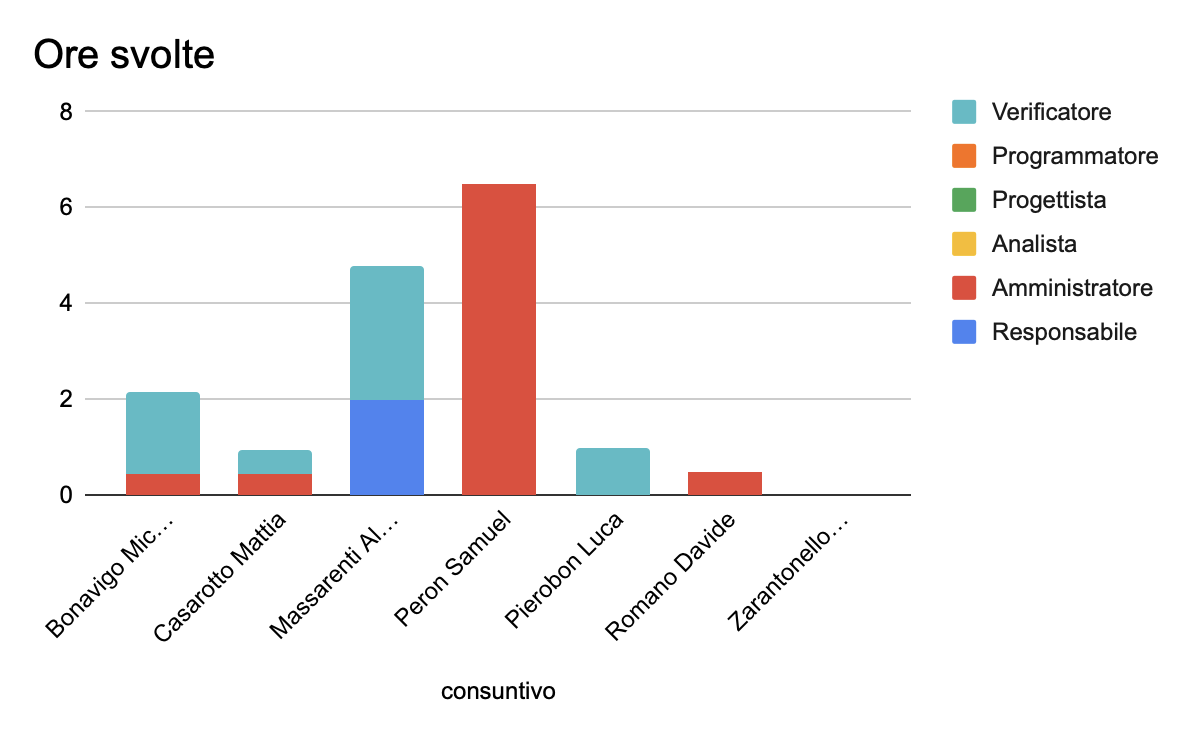
\includegraphics[width=12cm]{img/ore-svolte.png}
\end{center}

\begin{table}[ht]
    \begin{tabularx}{\linewidth}{X|l|l}
    \rowcolor{gray!30}& Ore & Costo \\
    \hline
    
    Responsabile & 3,9 & € 117,00 \\
    \rowcolor{gray!10}Amministratore & 1 & € 20,00 \\
    Analista & 28,55 & € 713,75 \\
    \rowcolor{gray!10}Progettista & 16 & € 400,00 \\
    Programmatore & 0 & € 0,00 \\
    \rowcolor{gray!10}Verificatore & 9,95 &€ 149,25 \\
    totale & 59,4 & € 1400,00 \\
    \end{tabularx}
    \caption{\label{costi-ruolo}Spartizione dei ruoli e ore svolte durante lo sprint}
\end{table}

Avendo quindi consumato €1400,00\footnote{Si veda tabella \ref{costi-ruolo}} del budget durante questo sprint, rimangono ancora a disposizione € 9906,50 per gli sprint seguenti.

\subsection{Trend e riflessioni}\label{subsec:trend}

\begin{figure}[H]
    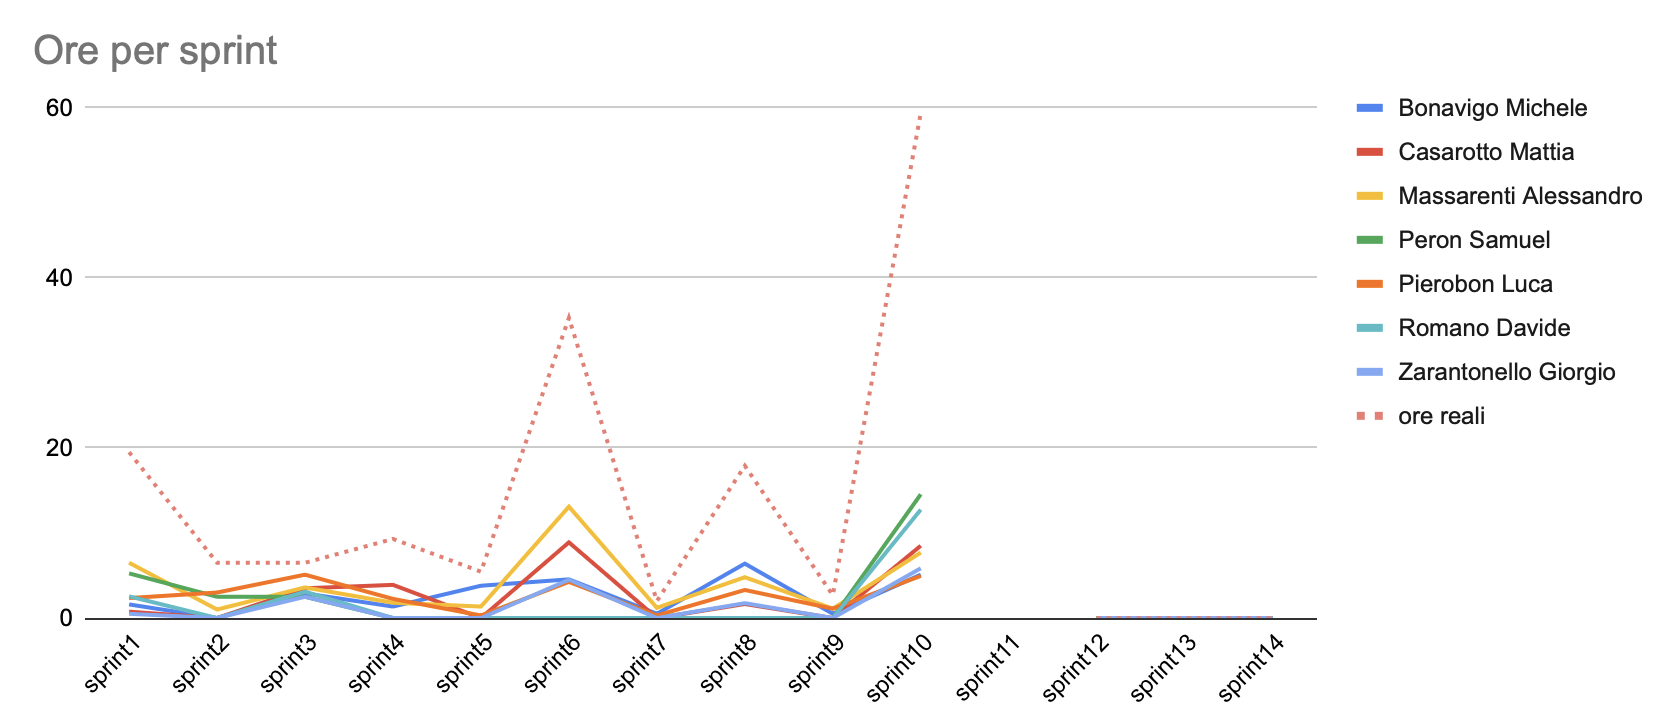
\includegraphics[width=\linewidth]{img/andamento.png}
    \caption{Andamento ore utilizzate nei vari sprint}\label{img:andamento}
\end{figure}

Durante questo sprint si è assistito ad una ripresa delle attività dopo il rallentamento dettato dal momento {\it{clou}} della sessione di esami. Tuttavia è stata riscontrata una collaborazione non uniforme da parte di tutti i membri del gruppo.

\subsection{Difficoltà e problemi di sprint}

Non ci sono state grandi difficoltà esterne durante questo sprint. Purtroppo però, come negli sprint appena precedenti, non siamo ancora riusciti a definire con il proponente il supporto hardware per i lampioni a cui dovremo fare fede.

Internamente, come difficoltà, si rimanda alla riflessione posta nella sezione \ref{subsec:trend}.

Queste verranno discusse in sede di preparazione del prossimo sprint.
